\section{Testiranje implementacije}
\label{sec:analiza_pravilnosti}
V tem poglavju predstavimo postopek, s katerim testiramo pravilnost implementacije algoritma ARRNO. Kljub izpeljavi algoritma v prejšnjem poglavju, je testiranje vseeno pomembno. S tem pokažemo, da smo algoritem pravilno generalizirali v višje dimenzije, da deluje za posebne primere točk (na primer, kadar imajo točke iz $\P$ enako eno ali več koordinat), ter da se v implementacijo ni prikradla kakšna napaka. 

\subsection{Ideja testiranja}
Naj bo $\P$ množica paroma nedominiranih točk in $\textbf{q}$ točka poizvedbe. Za vsak $r \geq 0$ velja
\[
S(\textbf{q}, r) \cap N(\P) \neq \varnothing \iff d(\textbf{q}, N(\P)) \leq r,
\]
kjer je $S(\textbf{q}, r)$ sfera s središčem v $\textbf{q}$ in radijem $r$.

% Osnovna ideja testiranja algoritma je torej, da za veliko naključno izbranih kombinacij množic $\P$ in poizvedbenih točk $\textbf{q}$ z algoritmom izračunamo razdaljo $r_\text{A}$. Nato pa za nek majhen $\delta > 0$ preverimo, ali obstajata preseka $S(\textbf{q}, r_\text{A} - \delta) \cap N(\P)$ in $S(\textbf{q}, r_\text{A} + \delta) \cap N(\P)$. Primer treh točk poizvedbe in ustrezajočih sfer v dveh dimenzijah vidimo na sliki~\ref{fig:test_example}.

Osnovna ideja testiranja algoritma je torej, da za naključno izbrano kombinacijo množice $\P$ in poizvedbene točke $\textbf{q}$ z algoritmom ARRNO izračunamo razdaljo $r_\text{A}$. Nato pa za nek majhen $\delta > 0$ preverimo, ali obstajata preseka $S(\textbf{q}, r_\text{A} - \delta) \cap N(\P)$ in $S(\textbf{q}, r_\text{A} + \delta) \cap N(\P)$. Primer treh točk poizvedbe in ustrezajočih sfer v dveh dimenzijah vidimo na sliki~\ref{fig:test_example}. Če velja da je presek $S(\textbf{q}, r_\text{A} - \delta) \cap N(\P)$ prazen in $S(\textbf{q}, r_\text{A} + \delta) \cap N(\P)$ neprazen, potem vemo, da je napaka algoritma največ $\delta$. Če to velja za majhen $\delta$ pri veliko naključnih množicah $\P$ in poizvedbenih točkah $\textbf{q}$, smo lahko o pravilnosti algoritma precej prepričani. 
\begin{figure}[ht]
  \centering
  \begin{tikzpicture}
    
    % Shade the non-dominated area (above and right)
    \fill[fillcol] 
        (0,5) -- (0,4) -- (0.5,4) -- 
        (0.5,2.5) -- (1.5,2.5) -- 
        (1.5,2) -- (2,2) -- 
        (2,1.5) -- (3.5,1.5) -- 
        (3.5,0.5) -- (4,0.5) -- 
        (4,0) -- (5,0) -- (5,5) -- cycle;
    \node at (3.75,3.75) {\( N(\P) \)};


    % Draw lines from each point (downward and leftward)
    \draw (0.5,4) -- (0.5,2.5);  
    \draw (0.5,4) -- (0,4);      

    \draw (1.5,2.5) -- (1.5,2);  
    \draw (1.5,2.5) -- (0.5,2.5);

    \draw (2,2) -- (2,1.5);      
    \draw (2,2) -- (1.5,2);      

    \draw (3.5,1.5) -- (3.5,0.5);
    \draw (3.5,1.5) -- (2,1.5);  

    \draw (4,0.5) -- (4,0);      
    \draw (4,0.5) -- (3.5,0.5);  

    % Nondominated points
    \fill (0.5,4) circle (2pt) node[above right] {\( \textbf{p}^1 \)};
    \fill (1.5,2.5) circle (2pt) node[above right] {\( \textbf{p}^2 \)};
    \fill (2,2) circle (2pt) node[above right] {\( \textbf{p}^3 \)};
    \fill (3.5,1.5) circle (2pt) node[above right] {\( \textbf{p}^4 \)};
    \fill (4,0.5) circle (2pt) node[above right] {\( \textbf{p}^5 \)};

    % Additional points q1, q2, q3
    \fill[nodecol2] (-0.4,4.2) circle (2pt) node[below left] {\( \textbf{q}^1 \)};
    \draw[nodecol, dashed] (-0.4,4.2) ++(0:0.45) arc[start angle=0, end angle=360, radius=0.45];    
    \draw[nodecol, dotted] (-0.4,4.2) ++(0:0.35) arc[start angle=0, end angle=360, radius=0.35];    


    
    \fill[nodecol2] (0.6,1) circle (2pt) node[below left] {\( \textbf{q}^2 \)};
    \draw[nodecol, dashed] (0.6,1) ++(0:1.3453624 + 0.05) arc[start angle=0, end angle=360, radius=1.3453624 + 0.05];    
    \draw[nodecol, dotted] (0.6,1) ++(0:1.3453624 - 0.05) arc[start angle=0, end angle=360, radius=1.3453624 - 0.05];    

    
    \fill[nodecol2] (2.5,1) circle (2pt) node[below left] {\( \textbf{q}^3 \)};
    \draw[nodecol, dashed] (2.5,1) ++(0:0.55) arc[start angle=0, end angle=360, radius=0.55];    
    \draw[nodecol, dotted] (2.5,1) ++(0:0.45) arc[start angle=0, end angle=360, radius=0.45];    
    
    % Draw lines to the nearest boundary of the non-dominated region
    \draw[nodecol2] (-0.4,4.2) -- (0,4.2);  % q1 to shaded region (horizontally right)
    \draw[nodecol2] (0.6, 1) -- (1.5,2);  % q2 to v (diagonal)
    \draw[nodecol2] (2.5,1) -- (2.5,1.5);  % q3 to shaded region (vertically up)

    % Draw axes
    \draw[->] (0,0) -- (5,0) node[midway, below] {\( f_1 \)};
    \draw[->] (0,0) -- (0,5) node[midway, left] {\( f_2 \)};
    
    % Draw a small dot at the origin
    \fill (0,0) circle (2pt);

\end{tikzpicture}

  \caption{Tri točke poizvedbe $\textbf{q}^1$, $\textbf{q}^2$, $\textbf{q}^3$, skupaj z njihovimi razdaljami do nedominiranega območja ter ustrezajočimi sferami $S(\textbf{q}, r_\text{A} + \delta)$ s črtkano črto in $S(\textbf{q}, r_\text{A} - \delta)$ s točkasto črto.}
  \label{fig:test_example}
\end{figure}


\subsection{Diskretizacija sfere}
Da lahko računamo presek sfere z $N(\P)$, sfero diskretiziramo. Diskretizacija sfere $S(\textbf{q}, r)$ je množica točk, označimo jo z $\Sigma(\textbf{q}, r, \varepsilon)$, ki ležijo na $S(\textbf{q}, r)$ in za katere velja
\[
\forall \textbf{x} \in S(\textbf{q}, r): \quad \min_{\textbf{s} \in \Sigma(\textbf{q}, r, \varepsilon)} ||\textbf{x} - \textbf{s}|| \leq \varepsilon.
\]
Presek med diskretno sfero $\Sigma(\textbf{q}, r, \varepsilon)$ in $N(\P)$ lahko nato izračunamo enostavno
\[
\Sigma(\textbf{q}, r, \varepsilon) \cap N(\P) = \{ \textbf{s} \in \Sigma(\textbf{q}, r, \varepsilon) \mid \textbf{s} \succeq 0 \land \neg  (\P \ggcurly \textbf{s}) \}.
\]

Za lažjo notacijo v tem razdelku brez škode za splošnost predpostavljamo, da je sfera centrirana v koordinatnem izhodišču. Prav tako diskretiziramo le pozitivni del sfere, torej točke ki imajo vse koordinate nenegativne, kar označimo s $\Sigma^+(\textbf{0}, r, \varepsilon)$. V trditvi~\ref{trditev1} namreč pokažemo, da to zadošča za preverjanje preseka z nedominiranim območjem. 

\begin{trditev} \label{trditev1}
Vse komponente vektorja od poljubne točke $\textbf{q} \notin N(\P)$ do njej najbližje točke $\textbf{z} \in N(\P)$ so nenegativne.
\end{trditev}

\begin{dokaz}
Predpostavimo, da za neko množico $\P$ in točko $\textbf{q} = (q_1, \dots, q_D) \notin N(\P)$ obstaja točka $\textbf{z} = (z_1, \dots, z_D) \in N(\P)$, ki je najbližja točki $\textbf{q}$ izmed točk v $N(\P)$ ter da je $i$-ta komponenta vektorja $\textbf{w} = (z_1 - q_1, \dots, z_D - q_D)$ od $\textbf{q}$ do $\textbf{z}$ negativna. 

Potem definirajmo vektor $\textbf{w'} = (z_1 - q_1, \dots 0, \dots, z_D - q_D)$, ki je enak vektorju $\textbf{w}$, le da ima $i$-to komponento enako $0$, ter novo točko $\textbf{z'} = \textbf{q} + \textbf{w'}$.
Za točko $\textbf{z'} = (z_1, \dots, z_{i-1}, q_i, z_{i+1}, \dots, z_D)$ potem velja $\textbf{z'} \succ \textbf{z}$, saj je po predpostavki $q_i > z_i$, vse ostale komponente pa so enake. Ker je $\textbf{z} \in N(\P)$ in $\textbf{z'} \succ \textbf{z}$, je torej tudi $\textbf{z'} \in N(\P)$. Prav tako je očitno, da je $d(\textbf{q}, \textbf{z'}) = || \textbf{w'} || < || \textbf{w} || = d(\textbf{q}, \textbf{z})$, torej $\textbf{z}$ ni najbližja točka $\textbf{q}$ izmed točk v $N(\P)$, kar nas privede v protislovje. 
\end{dokaz}


Preprost način za konstrukcijo diskretne sfere $\Sigma^+(\textbf{0}, r, \varepsilon)$ je, da diskretiziramo površino sferi očrtane kocke $\Gamma^+(\textbf{0}, r, \varepsilon)$, nato pa točke projeciramo na sfero, kot je vidno na sliki~\ref{fig:constructing_sphere}.
\begin{figure}[ht]
    \begin{subfigure}{0.49\textwidth}
        \centering
        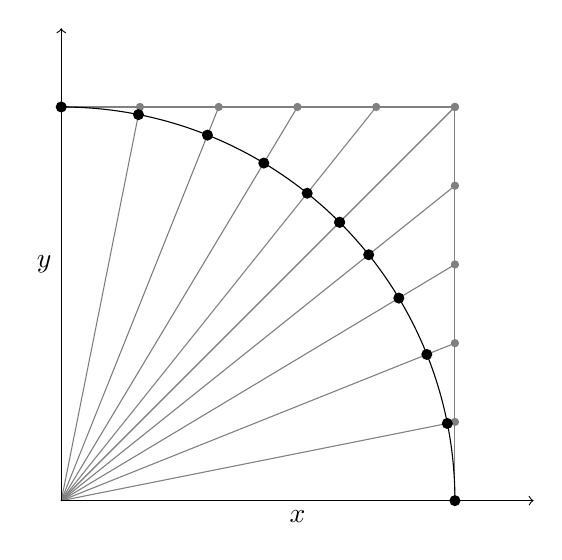
\begin{tikzpicture}

    \draw[gray] (5,0) -- (5,5);
    \draw[gray] (0,5) -- (5,5);

    \foreach \x in {0,1,2,3,4,5} {
        \draw[gray] (\x,5) -- (0,0);    
        \draw[gray] (5,\x) -- (0,0);    
        \fill[gray] (\x,5) circle (1.5pt);
        \fill[gray] (5,\x) circle (1.5pt);

        \pgfmathsetmacro{\r}{sqrt(\x*\x + 25)}
        \pgfmathsetmacro{\projx}{\x / \r * 5}
        \pgfmathsetmacro{\projy}{5 / \r * 5}

        \fill (\projx,\projy) circle (2pt);
        \fill (\projy,\projx) circle (2pt); 
    }

    \draw (5,0) arc[start angle=0, end angle=90, radius=5];    

    % Draw axes
    \draw[->] (0,0) -- (6,0) node[midway, below] {\( x \)};
    \draw[->] (0,0) -- (0,6) node[midway, left] {\( y \)};
\end{tikzpicture}

        \caption{Diskretizacija roba kocke in projekcija na sfero v dveh dimenzijah.}
        \label{fig:constructing_sphere_1}
    \end{subfigure}
    \hfill
    \begin{subfigure}{0.49\textwidth}
        \centering
        \tdplotsetmaincoords{70}{110}

\begin{tikzpicture}[scale=4,tdplot_main_coords]
\coordinate (O) at (0,0,0);
\draw[-stealth] (0,0,0) -- (1.2,0,0) node[anchor=north east]{$x$};
\draw[-stealth](0,0,0) -- (0,1.2,0) node[anchor=north west]{$y$};
\draw[-stealth] (0,0,0) -- (0,0,1.2) node[anchor=south]{$z$};

\draw[gray] (1,0,0) -- (1,1,0);
\draw[gray] (1,0,0) -- (1,0,1);
\draw[gray] (0,1,0) -- (1,1,0);
\draw[gray] (0,1,0) -- (0,1,1);
\draw[gray] (0,0,1) -- (1,0,1);
\draw[gray] (0,0,1) -- (0,1,1);
\draw[gray] (1,1,1) -- (0,1,1);
\draw[gray] (1,1,1) -- (1,0,1);
\draw[gray] (1,1,1) -- (1,1,0);

\foreach \x in {0,0.2,0.4,0.6,0.8,1} {
    \foreach \y in {0,0.2,0.4,0.6,0.8,1} {
        %\fill[gray] (\x,\y,1) circle (0.4pt);
        %\fill[gray] (\x,1,\y) circle (0.4pt);
        %\fill[gray] (1,\x,\y) circle (0.4pt);
        
        \pgfmathsetmacro{\r}{sqrt(\x*\x + \y*\y + 1)}
        \pgfmathsetmacro{\projx}{\x / \r}
        \pgfmathsetmacro{\projy}{\y / \r}
        \pgfmathsetmacro{\projz}{1 / \r}

        \draw[gray] (\projx,\projy,\projz) -- (\x,\y,1);
        \draw[gray] (\projx,\projz,\projy) -- (\x,1,\y);
        \draw[gray] (\projz,\projx,\projy) -- (1,\x,\y);

        \fill (\projx,\projy,\projz) circle (0.4pt);
        \fill (\projx,\projz,\projy) circle (0.4pt);
        \fill (\projz,\projx,\projy) circle (0.4pt);

        
    }
}






\tdplotsetthetaplanecoords{90}
% \tdplotdrawarc[tdplot_rotated_coords]{(0,0,0)}{0.5}{80}%
% {90}{anchor=west}{$d\phi_1$}
\draw[gray, dashed,tdplot_rotated_coords] (1,0,0) arc (0:90:1);

\draw[gray, dashed] (1,0,0) arc (0:90:1);

\tdplotsetthetaplanecoords{0}
\draw[gray, dashed,tdplot_rotated_coords] (1,0,0) arc (0:90:1);


\end{tikzpicture}
        \caption{Diskretizacija roba kocke in projekcija na sfero v treh dimenzijah.}
        \label{fig:constructing_sphere_2}
    \end{subfigure}
    \caption{Prikaz delovanja algoritma za diskretizacijo sfere v dveh in treh dimenzijah.}
    \label{fig:constructing_sphere}
\end{figure}

Pozitivni del hiperkocke v $D$ dimenzijah diskretiziramo tako, da združimo diskretizacijo vsake izmed $D$ pozitivnih stranic hiperkocke. Diskretizacija $i$-te stranice hiperkocke s stranico dolžine $r$ na $k+1$ točk je množica točk 
\[
\left\{0, \frac{1}{k}r, \frac{2}{k}r, \dots, \frac{k-1}{k}r, r\right\}^{i-1} \times \left\{ r \right\} \times \left\{0, \frac{1}{k}r, \frac{2}{k}r, \dots, \frac{k-1}{k}r, r\right\}^{D-i}.
\]
Torej je
\[
\Gamma^+(\textbf{0}, r, \varepsilon) = \bigcup_{i=1}^D \left\{0, \frac{1}{k}r, \frac{2}{k}r, \dots, \frac{k-1}{k}r, r\right\}^{i-1} \times \left\{ r \right\} \times \left\{0, \frac{1}{k}r, \frac{2}{k}r, \dots, \frac{k-1}{k}r, r\right\}^{D-i},
\]
iz česar pa enostavno dobimo diskretizacijo sfere $\Sigma^+(\textbf{q}, r, \varepsilon)$, tako da za vsako točko $\gamma \in \Gamma^+(\textbf{0}, r, \varepsilon)$ izračunamo njeno projekcijo $\sigma$ na sfero 
\[
\sigma = \frac{\gamma}{|| \gamma ||} r.
\]
Potrebno je le še določiti gostoto mreže, torej dolžino delitvenega intervala $\frac{r}{k}$. V dimenziji $D$ najbolj oddaljena točka $\textbf{x}$ od diskretne mreže leži ravno na sredini med točkami mreže, kot vidimo na sliki~\ref{fig:proof_h}, z maksimalno razdaljo enako 
\[
d_{\max} = \sqrt{(D-1)\frac{r^2}{(2k)^2}} = \frac{r}{2k}\sqrt{D-1}.
\]
Ker želimo da je $d_{\max} \leq \varepsilon$ mora veljati 
\[
\frac{r}{k} \leq \frac{2\varepsilon}{\sqrt{D-1}},
\]
kar velja za
\[
k = \left\lceil \frac{r \sqrt{D-1}}{2\varepsilon} \right\rceil.
\]
\begin{figure}[ht]
    \begin{subfigure}{0.32\textwidth}
        \centering
        \begin{tikzpicture}
    \draw[gray, dashed] (-0.5, 1) -- (2.5, 1) node[midway, below] {$\frac{r}{k}$};    \draw[line width=0.3mm, nodecol2] (0, 1) -- (1, 1);      

    \fill (0,1) circle (2pt);
    \fill (2,1) circle (2pt);
    \fill[nodecol2] (1,1) circle (2pt) node[above right] {\( \textbf{x} \)};

\end{tikzpicture}

        %\caption{.}
        %\label{fig:proof_h2d}
    \end{subfigure}
    \hfill
    \begin{subfigure}{0.32\textwidth}
        \centering
        \begin{tikzpicture}

    \draw[gray, dashed] (-0.5, 0) -- (2.5, 0) node[midway, below] {$\frac{r}{k}$};    
    \draw[gray, dashed] (-0.5, 2) -- (2.5, 2);      
    \draw[gray, dashed] (0, -0.5) -- (0, 2.5);      
    \draw[gray, dashed] (2, -0.5) -- (2, 2.5);      

    % Draw a small dot at the origin
    \fill (0,0) circle (2pt);
    \fill (0,2) circle (2pt);
    \fill (2,0) circle (2pt);
    \fill (2,2) circle (2pt);

    \draw (0, 0) -- (1, 0);      
    \draw (1, 0) -- (1, 1);      
    
    \fill[nodecol2] (1,1) circle (2pt) node[above right] {\( \textbf{x} \)};
    \draw[line width=0.3mm, nodecol2] (1, 1) -- (0, 0);


\end{tikzpicture}

        %\caption{.}
        %\label{fig:proof_h3d}
    \end{subfigure}
    \hfill
    \begin{subfigure}{0.32\textwidth}
        \centering
        \tdplotsetmaincoords{70}{100}

\begin{tikzpicture}[scale=2,tdplot_main_coords]

\draw[gray, dashed] (1,-0.2,0) -- (1,1.2,0) node[midway, below] {$\frac{r}{k}$};
\draw[gray, dashed] (0,-0.2,0) -- (0,1.2,0);
\draw[gray, dashed] (1,0,-0.2) -- (1,0,1.2);
\draw[gray, dashed] (0,0,-0.2) -- (0,0,1.2);
\draw[gray, dashed] (-0.2,1,0) -- (1.2,1,0);
\draw[gray, dashed] (-0.2,0,0) -- (1.2,0,0);
\draw[gray, dashed] (0,1,-0.2) -- (0,1,1.2);
\draw[gray, dashed] (-0.2,0,1) -- (1.2,0,1);
\draw[gray, dashed] (0,-0.2,1) -- (0,1.2,1);
\draw[gray, dashed] (1.2,1,1) -- (-0.2,1,1);
\draw[gray, dashed] (1,1.2,1) -- (1,-0.2,1);
\draw[gray, dashed] (1,1,1.2) -- (1,1,-0.2);

\foreach \x in {0, 1} {
    \foreach \y in {0, 1} {
        \foreach \z in {0, 1} {
            \fill (\x,\y,\z) circle (1pt);
        }
    }
}

\draw (1,0,0) -- (1,0.5,0);
\draw (1,0.5,0) -- (0.5,0.5,0);
\draw (0.5,0.5,0.5) -- (0.5,0.5,0);

\draw[line width=0.3mm, nodecol2] (0.5,0.5,0.5) -- (1, 0, 0);
\fill[nodecol2] (0.5,0.5,0.5) circle (1pt) node[above right] {\( \textbf{x} \)};


\end{tikzpicture}

        %\caption{.}
        %\label{fig:proof_h4d}
    \end{subfigure}
    \caption{Primeri diskretizacij dela stranice dvodimenzionalne kocke na levi, tridimenzionalne kocke na sredini in štiridimenzionalne kocke na desni, skupaj s točko $\textbf{x}$, ki je od diskretizacije najbolj oddaljena.}
    \label{fig:proof_h}
\end{figure}

Za dobro izbiro $k$ torej velja, da je vsaka točka $\textbf{x}$ iz površine hiperkocke, največ za $\varepsilon$ oddaljena od diskretizacije. 
\begin{trditev}
\label{trditev:projekcija}
Za poljubni $D$-dimenzionalni točki $A$ in $B$ iz zunanjosti sfere in njuni projekciji na sfero $A'$ in $B'$ velja
\[
|| A' - B' || \leq || A - B ||. 
\]
\end{trditev}
\begin{dokaz}
Osredotočimo se lahko le na ravnino, ki gre skozi izhodišče sfere in točki $A$ in $B$, ki je prikazana na sliki~\ref{fig:sphere_contraction}. Naj bo $\theta$ kot med točkama $A$ in $B$ v tej ravnini. Po kosinusnem izreku je potem 
\[
||A' - B'||^2 = 2r^2 - 2r^2 \cos \theta,
\]
kjer je $r$ radij sfere in
\[
||A - B||^2 = (r + r_A)^2 + (r + r_B)^2 - 2(r + r_A) (r + r_B) \cos \theta,
\]
kjer sta $r + r_A$ in $r + r_B$ razdalji med izhodiščem sfere in točko $A$ oziroma $B$. Potem je
\[
||A - B||^2 - ||A' - B'||^2 = rr_A (2 - 2 \cos \theta) + rr_B (2 - 2 \cos \theta) + r_A^2 + r_B^2 - 2 r_A r_B \cos \theta
\]
Ker sta $r_A, r_B \geq 0$ očitno velja $rr_A (2 - 2 \cos \theta) \geq 0$ in $rr_B (2 - 2 \cos \theta) \geq 0$. Po kosinusnem izreku enako velja za $r_A^2 + r_B^2 - 2 r_A r_B \cos \theta$, saj je to ravno kvadrat dolžine nasprotne stranice trikotnika s stranicama $r_A$ in $r_B$ ter kotom $\theta$ med njima. Ker je torej $||A - B||^2 \geq ||A' - B'||^2$ je tudi $||A - B|| \geq ||A' - B'||$.
\begin{figure}[ht]
  \centering
  \begin{tikzpicture}

    \draw[gray] (0,0) -- (2.8284,2.8284);
    \draw[gray] (0,0) -- (2.058,3.43) node[midway, above] {\( r \)};
    
    \draw[gray] (2.8284,2.8284) -- (3.5, 3.5) node[midway, above, left] {\( r_B \)};
    \draw[gray] (2.058,3.43) -- (3,5) node[midway, above, left] {\( r_A \)};

    \draw (4,0) arc[start angle=0, end angle=90, radius=4];  
    \draw (2,2) arc[start angle=45, end angle=59.03, radius=2.828];  

    \draw[gray, dashed] (3,5) -- (3.5, 3.5);
    \draw[gray, dashed] (2.058,3.43) -- (2.8284,2.8284);

    \draw (1.55,2) node {\( \theta \)};


    \fill (3,5) circle (2pt) node[above right] {\( A \)};
    \fill (3.5, 3.5) circle (2pt) node[above right] {\( B \)};

    \fill (2.058,3.43) circle (2pt) node[above right] {\( A' \)};
    \fill (2.8284,2.8284) circle (2pt) node[right] {\( B' \)};


    % Draw axes
    \draw[->] (0,0) -- (6,0) node[midway, below] {\( x \)};
    \draw[->] (0,0) -- (0,6) node[midway, left] {\( y \)};
\end{tikzpicture}

  \caption{Slika prikazuje točki $A$ in $B$, njuni projekciji na sfero $A'$ in $B'$ ter razdalje $r$, $r_A$ in $r_B$.}
  \label{fig:sphere_contraction}
\end{figure}
\end{dokaz}

Po trditvi~\ref{trditev:projekcija} torej tudi za diskretizacijo sfere velja, da je vsaka točka $\textbf{x}$ iz površine sfere največ za $\varepsilon$ oddaljena od njene diskretizacije. 
\subsection{Gostota diskretizacije}
Za dani $\delta$ želimo izbrati tak $\varepsilon$, da je gostota diskretizacije dovolj velika in velja
\[
d(\textbf{q}, N(\P)) \leq r \implies \Sigma(\textbf{q}, r + \delta, \varepsilon) \cap N(\P) \neq \varnothing.
\]
Sicer bi se nam lahko zgodilo, da zaradi nesrečne izbire diskretizacije v preseku ne bi bilo nobene točke, kot je vidno na sliki~\ref{fig:determining-epsilon3}.
\begin{figure}[ht]
  \centering
  \begin{tikzpicture}
    
    % Shade the non-dominated area (above and right)
    \fill[fillcol] 
        (-2,4) -- (-2,3) -- (0.1,3) -- 
        (0.1, 0) -- (3,0) -- 
        (3, -1) -- (4,-1) -- (4,4) -- cycle;
    \node at (3,3) {\( N(\P) \)};


    % Draw lines from each point (downward and leftward)
    \draw (0.1,3) -- (-2,3);  
    \draw (0.1,3) -- (0.1,0);      

    \draw (3,0) -- (0.1,0);  
    \draw (3,0) -- (3, -1);  

    
    \fill (0.1,3) circle (2pt) node[above right] {\( \textbf{p}^i \)};
    \fill (3,0) circle (2pt) node[above right] {\( \textbf{p}^{i+1} \)};
    
     \fill (-2,-1) circle (2pt) node[above right] {\( \textbf{q} \)};
    \draw[nodecol, dashed] (-2,-1) -- (0.5,-1) node[midway, above] {$r$};  
    \draw[nodecol, dashed] (-2,-1) -- (-2,1.5);  
    \draw[nodecol] (0.5,-1) arc[start angle=0, end angle=90, radius=2.5];

    \foreach \x in {0, 18, 36, 54, 72, 90} {
        \fill[nodecol] ({-2 + 2.5* cos(\x)}, {-1 + 2.5* sin(\x)}) circle (2pt);
    }

    


\end{tikzpicture}

  \caption{Gostota diskretizacije sfere $S(\textbf{q}, r)$ je premajhna, da bi kakšna izmed točk diskretizacije $\Sigma(\textbf{q}, r, \varepsilon)$ padla v nedominirano območje $N(\P)$, kljub temu da je $d(\textbf{q}, N(\P)) < r$.}
  \label{fig:determining-epsilon3}
\end{figure}
Očitno je, da bomo za čim manjši $\delta$ potrebovali tem gostejšo diskretizacijo sfere. 
\begin{trditev}
\label{trditev:dokaz_pravilnosti}
Za izbiro $\varepsilon \leq \frac{\delta}{\sqrt{D}}$ velja
\[
d(\textbf{q}, N(\P)) \leq r \implies \Sigma(\textbf{q}, r + \delta, \varepsilon) \cap N(\P) \neq \varnothing.
\]
\end{trditev}
\begin{dokaz}
Oglejmo si sliko~\ref{fig:determining-epsilon1}, kjer vidimo primer točke $\textbf{q}$, ki je do najbližje točke $\textbf{v} \in N(\P)$ oddaljena za $r$. Prikazan je tudi pozitivni del sfere $S(\textbf{q}, r + \delta)$ s središčem v $\textbf{q}$ in radijem $r + \delta$ ter pozitivni del sfere $S(\textbf{v}, \delta)$ s središčem v $\textbf{v}$ in radijem $\delta$. Po trikotniški neenakosti sledi, da so vse točke na $S(\textbf{q}, r + \delta)$ od $\textbf{v}$ oddaljene več ali enako $\delta$. 
\begin{figure}[ht]
  \centering
  \begin{tikzpicture}
    
    % Shade the non-dominated area (above and right)
    \fill[fillcol] 
        (-2,4) -- (-2,3) -- (0,3) -- 
        (0, 0) -- (3,0) -- 
        (3, -1) -- (4,-1) -- (4,4) -- cycle;
    \node at (3,3) {\( N(\P) \)};


    % Draw lines from each point (downward and leftward)
    \draw (0,3) -- (-2,3);  
    \draw (0,3) -- (0,0);      

    \draw (3,0) -- (0,0);  
    \draw (3,0) -- (3, -1);  

    
    \fill (0,3) circle (2pt) node[above right] {\( \textbf{p}^i \)};
    \fill (3,0) circle (2pt) node[above right] {\( \textbf{p}^{i+1} \)};
    \fill (0,0) circle (2pt) node[above left] {\( \textbf{v}\)};
    
     \fill (-2,-1) circle (2pt) node[above right] {\( \textbf{q} \)};
    \draw[nodecol, dashed] (-2,-1) -- (1.23606798,-1) node[midway, above] {$r + \delta$};  
    \draw[nodecol, dashed] (-2,-1) -- (-2,2.23606798);  
    % \draw[nodecol, dashed] (0.23606798,-1) -- (1.23606798,-1) node[midway, above] {$\delta$};
    \draw[nodecol] (1.23606798,-1) arc[start angle=0, end angle=90, radius=3.23606798];    
    % \draw[nodecol, dashed] (0.23606798,-1) arc[start angle=0, end angle=90, radius=2.23606798];    
    \draw[blue, dashed] (-2,-1) -- (0,0) node[midway, above] {$r$};
    \draw[blue] (0.8944272,0.4472136) -- (0,0) node[midway, above] {$\delta$};
    \draw[blue] (1, 0) arc[start angle=0, end angle=90, radius=1];    
    % \fill[blue] (0.70710678,0.70710678) circle (1pt) node[left] {$\overline{\textbf{s}}$};
    
    
    % \draw[gray, dashed] (1,1) -- (0,0);
    % \fill[gray] (0.73295,0.73295) circle (1pt) node[right] {\( \textbf{s} \)};

    % \draw[blue, dashed] (0.707106781,0.707106781) circle (0.707106781); 



\end{tikzpicture}

  \caption{Slika prikazuje primer točke $\textbf{q}$ ter njej najbližjo točko iz $N(P)$, točko $\textbf{v}$. Z oranžno barvo je prikazana testna sfera  $S(\textbf{q}, r + \delta)$, z modro barvo pa $S(\textbf{v}, \delta)$.}
  \label{fig:determining-epsilon1}
\end{figure}

Skozi $\textbf{v}$ nato potegnemo premico $l$ pod kotom $45^\circ$ na vse koordinatne osi, ki seka $S(\textbf{v}, \delta)$ v točki $\textbf{s}$, kot vidimo na sliki~\ref{fig:determining-epsilon2}. Po podobnem razmisleku, kot na sliki~\ref{fig:proof_h} je jasno, da je vektor od $\textbf{v}$ do $\textbf{s}$ enak $(\frac{\delta}{\sqrt{D}}, \dots, \frac{\delta}{\sqrt{D}})$. Torej krogla $B(\textbf{s}, \frac{\delta}{\sqrt{D}})$ v celoti leži znotraj $N(\P)$. Naj bo $I = S(\textbf{v}, \delta) \cap B(\textbf{s}, \frac{\delta}{\sqrt{D}})$ del sfere $S(\textbf{v}, \delta)$, ki leži znotraj krogle $B(\textbf{s}, \frac{\delta}{\sqrt{D}})$. Množica $I \subset N(\P)$ vsebuje vse točke iz $S(\textbf{v}, \delta)$, ki so od $\textbf{s}$ oddaljene manj kot $\frac{\delta}{\sqrt{D}}$. Torej pri vsaki diskretizaciji $S(\textbf{v}, \delta)$ z $\varepsilon \leq \frac{\delta}{\sqrt{D}}$ obstaja točka diskretizacije, ki leži v $I$ torej leži tudi v $N(\P)$.
\begin{figure}[ht]
  \centering
  \begin{tikzpicture}
    
    % Shade the non-dominated area (above and right)
    \fill[fillcol] 
        (-2,4) -- (-2,3) -- (0,3) -- 
        (0, 0) -- (3,0) -- 
        (3, -1) -- (4,-1) -- (4,4) -- cycle;
    \node at (3,3) {\( N(\P) \)};


    % Draw lines from each point (downward and leftward)
    \draw (0,3) -- (-2,3);  
    \draw (0,3) -- (0,0);      

    \draw (3,0) -- (0,0);  
    \draw (3,0) -- (3, -1);  

    
    \fill (0,3) circle (2pt) node[above right] {\( \textbf{p}^i \)};
    \fill (3,0) circle (2pt) node[above right] {\( \textbf{p}^{i+1} \)};
    \fill (0,0) circle (2pt) node[above left] {\( \textbf{v}\)};
    \fill (-2,-1) circle (2pt) node[above right] {\( \textbf{q} \)};
    
    \draw[nodecol, dashed] (-2,-1) -- (1.23606798,-1);  
    \draw[nodecol, dashed] (-2,-1) -- (-2,2.23606798);  
    % \draw[nodecol, dashed] (0.23606798,-1) -- (1.23606798,-1) node[midway, above] {$\delta$};
    \draw[nodecol] (1.23606798,-1) arc[start angle=0, end angle=90, radius=3.23606798];    
    \draw[blue, dashed] (-2,-1) -- (0,0);
    % \draw[blue] (0.8944272,0.4472136) -- (0,0) node[midway, above] {$\delta$};
    \draw[blue] (1, 0) arc[start angle=0, end angle=90, radius=1];    
    \fill[blue] (0.70710678,0.70710678) circle (1pt) node[left] {$\textbf{s}$};
    
    
    \draw[gray, dashed] (0,0) -- (4,4);
    \draw[gray, dashed] (-1,-1) -- (0,0) node[midway, right] {\( l \)};
    \draw[blue, dashed] (0.707106781,0.707106781) circle (0.707106781); 

    \fill[nodecol] (0.73295,0.73295) circle (1pt) node[right] {\( \textbf{s}' \)};
    \draw[nodecol, dashed]  (0.73295,0.73295) circle (0.707106781);    



\end{tikzpicture}

  \caption{S sivo črto je prikazana premica $l$, ki gre skozi točko $\textbf{v}$, ter seka modro oziroma oranžno sfero v točkah $\textbf{s}$ ter $\textbf{s}'$. Okrog točk $\textbf{s}$ in $\textbf{s}'$ sta prikazani sferi z radijem $\frac{\delta}{\sqrt{D}}$.}
  \label{fig:determining-epsilon2}
\end{figure}

Podobno lahko definiramo točko $\textbf{s}'$, ki je na presečišču premice $l$ in sfere $S(\textbf{q}, r + \delta)$. Ker je del sfere $S(\textbf{q}, r + \delta)$, ki je znotraj $N(\P)$, kvečjemu dlje od $\textbf{v}$ kot $S(\textbf{v}, \delta)$, bo po enakem razmisleku veljalo, da je diskretizacija z $\varepsilon \leq \frac{\delta}{\sqrt{D}}$ dovolj natančna tudi za $S(\textbf{q}, r + \delta)$.

\end{dokaz}


\subsection{Testiranje}
Naj bo $r_{\text{A}}$ z algoritmom izračunana razdalja med nedominiranim območjem dane množice $\P$ ter poizvedbene točke $\textbf{q}$. Za nek majhen $\delta$ bi radi pokazali da velja $d(\textbf{q}, N(\P)) - \delta \leq r_\text{A} \leq d(\textbf{q}, N(\P)) + \delta$. 

\subsubsection{Spodnja meja}
Izberemo $\varepsilon = \frac{\delta}{\sqrt{D}}$ in preverimo presek $\Sigma(\textbf{q}, r_{\text{A}} + \delta, \varepsilon) \cap N(\P)$. Če presek vsebuje kako točko, vemo da velja $d(\textbf{q}, N(\P)) \leq r_\text{A} + \delta$ oziroma $d(\textbf{q}, N(\P)) - \delta \leq r_\text{A}$. Sicer pa po trditvi~\ref{trditev:dokaz_pravilnosti} vemo, da je $d(\textbf{q}, N(\P)) > r_\text{A}$ torej algoritem ne deluje pravilno. 

\subsubsection{Zgornja meja}
Iz trditve~\ref{trditev:dokaz_pravilnosti} po kontrapoziciji velja
\[
\Sigma(\textbf{q}, r, \varepsilon) \cap N(\P) = \varnothing \implies d(\textbf{q}, N(\P)) > r - \delta,
\]
pri izbiri $\varepsilon = \frac{\delta}{\sqrt{D}}$. Presek $\Sigma(\textbf{q}, r_\text{A}, \varepsilon) \cap N(\P)$ ob pravilnem delovanju algoritma ni nujno prazen, zato preverimo presek $\Sigma(\textbf{q}, r_\text{A} - \mu, \varepsilon') \cap N(\P)$, kjer je $\mu = \frac{\delta}{10^6}$, $\varepsilon' = \frac{\delta'}{\sqrt{D}}$ in $\delta' = \delta - \mu$. Če presek ni prazen, vemo da algoritem deluje narobe, sicer pa napako omejimo na
\[
r_\text{A} - \mu - (\delta - \mu) < d(\textbf{q}, N(\P)),
\]
iz česar sledi
\[
r_\text{A} \leq d(\textbf{q}, N(\P)) + \delta.
\]

\subsubsection{Rezultati testiranja}
Algoritem testiramo za dimenzije 3, 4, 5 in 6. Pri vsaki dimenziji ponovimo 100 poskusov z različnimi množicami $\P$ in točkami $\textbf{q}$. Da dobimo množico $\P$, naključno izberemo 100 točk iz $[0, 1]^D$ in odstranimo dominirane. Da dobimo točko $\textbf{q}$, prav tako naključno izbiramo točke iz $[0, 1]^D$, dokler $\P$ točke ne dominira. Nato z algoritmom ARRNO izračunamo razdaljo $r_\text{A}$ med točko $\textbf{q}$ ter nedominiranim območjem množice $\P$. Rezultate testiramo za čim manjše vrednosti $\delta$, kolikor nam omogočajo zmogljivosti strojne opreme. Ker za preverjanje preseka $\Sigma(\textbf{q}, r, \varepsilon) \cap N(\P)$ preverimo vsako kombinacijo točk iz $\Sigma(\textbf{q}, r, \varepsilon)$ in iz $\P$, za to potrebujemo $O(|\Sigma(\textbf{q}, r, \varepsilon)| \cdot |\P|)$ primerjav. Vrednost $\delta$ izberemo v odvisnosti od $r_\text{A}$, da je število točk diskretizacije vedno enako. Prav tako za višje dimenzije izberemo večji $\delta$, saj se število točk diskretizacije z dimenzijo veča. Tabela~\ref{tab:vrednosti_delta} prikazuje vrednosti $\delta$ in velikost diskretizacije sfere za različne dimenzije.
\begin{table}[htb]
    \centering
    \begin{tabular}{c r r}
        dimenzija & vrednost $\delta$ & št.~točk diskretizacije  \\
        \hline
        3 & $0.001 \cdot r_\text{A}$ & $\sim 4.5 \cdot 10^6$ \\
        4 & $0.01 \cdot r_\text{A}$ & $\sim 21.6 \cdot 10^6$ \\
        5 & $0.05 \cdot r_\text{A}$ & $\sim 25.5 \cdot 10^6$ \\
        6 & $0.2 \cdot r_\text{A}$ & $\sim 9.9 \cdot 10^6$ \\
    \end{tabular}
    \caption{Tabela prikazuje izbrane vrednosti za $\delta$ pri različnih dimenzijah, povprečno število točk diskretizacije sfere z izbranim $\delta$ ter povprečno število vpetih točk.}
    \label{tab:vrednosti_delta}
\end{table}

Da testiramo tudi primer, ko imata dve ali več točk kakšno izmed koordinat enako, vse poskuse ponovimo, le da tokrat točke za množico $\P$ izbiramo naključno iz $\{0.1, 0.2, \dots, 0.9, 1 \}^D$. Tako je verjetnost, da imata dve točki neko koordinato enako precej večja. Poskuse prav tako ponovimo še za primer, ko točka $\textbf{q} \notin [0, 1]^D$. Tokrat jo naključno izberemo iz množice $[-1, 1]^D \setminus [0, 1]^D$. 

Skupaj torej naključno ustvarimo $800$ testnih problemov, na katerih preverimo delovanje. Testiranje na namiznem računalniku s 16 GB pomnilnika
in frekvenco procesorja 3,60 GHz traja nekaj dni. V vseh primerih algoritem ARRNO deluje pravilno, kar kaže na to, da je zasnova in implementacija pravilna.  

